\begin{center}
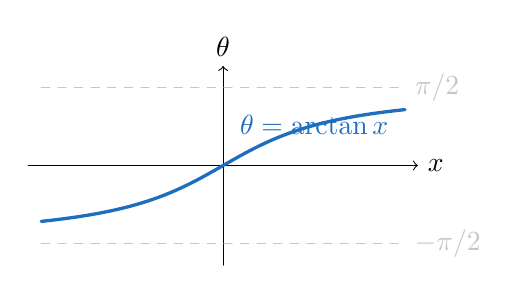
\begin{tikzpicture}[scale=1.1, line cap=round, line join=round]
  \definecolor{trigblue}{RGB}{30,110,190}
  \draw[->] (-2.25,0)--(2.25,0) node[right] {$x$};
  \draw[->] (0,-1.15)--(0,1.15) node[above] {$\theta$};
  \draw[gray!45,dashed] (-2.1,0.9)--(2.1,0.9) node[right] {$\pi/2$};
  \draw[gray!45,dashed] (-2.1,-0.9)--(2.1,-0.9) node[right] {$-\pi/2$};
  \draw[very thick,trigblue,domain=-2.1:2.1,samples=90]
    plot ({\x},{0.9*atan(\x)/90});
  \node[trigblue] at (1.05,0.47) {$\theta=\arctan x$};
\end{tikzpicture}
\end{center}


\begin{definitionbox}{Definition}
\begin{definition}[Inverse tangent]
\label{def:inverse-tangent}
The \emph{inverse tangent} function is the inverse of tangent after tangent is
restricted to the interval $(-\pi/2,\pi/2)$. It is denoted by $\arctan$ or
$\tan^{-1}$ and has domain $\mathbb{R}$ and range $(-\pi/2,\pi/2)$.
\[
  \arctan x=\theta
  \quad\Longleftrightarrow\quad
  \tan\theta=x
  \quad\text{and}\quad
  -\frac{\pi}{2}<\theta<\frac{\pi}{2}.
\]
\end{definition}
\end{definitionbox}
\begin{remark*}[Standard quantified statement]
For every admissible input satisfying the hypotheses of the statement, the
displayed definition or assertion holds in the stated domain.
\end{remark*}

\begin{remark*}[Interpretation]
The statement records the named trigonometric object or identity together with
its intended domain of use.
\end{remark*}

\begin{remark*}[Domain and range]
The tangent function has domain
$\mathbb{R}\setminus\{\pi/2+k\pi:k\in\mathbb{Z}\}$ and range $\mathbb{R}$.
The inverse tangent function reverses the principal restricted tangent
function, so its domain is $\mathbb{R}$ and its range is
$(-\pi/2,\pi/2)$.
\end{remark*}
\begin{dependencies}
\begin{itemize}
  \item \hyperref[def:extended-tangent]{Extended tangent}
  \item \hyperref[def:radian-measure]{Radian measure}
\end{itemize}
\end{dependencies}

\begin{theorembox}{Theorem}
\begin{theorem}[Principal inverse tangent identities]
\label{thm:inverse-tangent-identities}
For every $x\in\mathbb{R}$,
\[
  \tan(\arctan x)=x.
\]
For every $\theta\in(-\pi/2,\pi/2)$,
\[
  \arctan(\tan\theta)=\theta.
\]
\end{theorem}
\end{theorembox}
\begin{remark*}[Interpretation]
The statement records the named trigonometric object or identity together with
its intended domain of use.
\end{remark*}

\begin{remark*}[Standard quantified statement]
$\forall x\in\mathbb{R}$, $\tan(\arctan x)=x$, and
$\forall \theta\in(-\pi/2,\pi/2)$, $\arctan(\tan\theta)=\theta$.
\end{remark*}
\begin{dependencies}
\begin{itemize}
  \item \hyperref[def:inverse-tangent]{Inverse tangent}
\end{itemize}
\end{dependencies}
